\documentclass[chaptersright]{informeutn}
\usepackage[utf8]{inputenc}
\usepackage{array}
\usepackage[table]{xcolor}
\usepackage{colortbl}
\usepackage{caption}
\usepackage{graphicx}
\usepackage{amsmath}
\usepackage{multirow}
\usepackage{float}
\usepackage{geometry}[a4paper,margin=2.5cm]
\newcommand{\widemargins}{
  \newgeometry{left=1.5cm,right=1.5cm,top=1.8cm,bottom=1.8cm}
}
\newcommand{\restoremargins}{\restoregeometry}

\materia{Dispositivos Electronicos I}
\titulo{Trabajo Practico N°5: TIRISTORES}
\comision{3R2}
\autores{Documentador y operador: Gaston Grasso 401892\\ Coordinador: Angelo Prieto 401012}
\fecha{14-10-2025}


\begin{document}
\maketitle
\tableofcontents

\chapter{Introduccion}

\chapter{SCR}
\section{Condición de disparo y corriente de mantenimiento}
\subsection{Actividad de laboratorio}

\begin{figure}[h]
    \centering
     \begin{tikzpicture}
        % Paths, nodes and wires:
        \draw (-6.38, 2) to[american resistor, l={$R_1$}] (-6.38, 4);
        \draw (-6.38, 1) to[american potentiometer] (-6.38, -1);
        \draw (-3.38, -0) to[american resistor, l={$R_G$}] (-5.38, -0);
        \draw (-2.88, -0) to[ammeter, l={$I_G$}] (-0.88, -0);
        \draw (-0.88, -0) to[normal open switch] (1.37, -0);
        \draw (2.154, 2.295) to[empty thyristor, mirror] (2.134, -0.905);
        \draw (2.154, 2.295) to[american resistor, l={$R_2$}] (2.154, 4.295);
        \draw (2.12, -3) to[ammeter, l={$I_{AK}$}] (2.134, -0.905);
        \draw (4.12, -1) to[voltmeter, l={$V_{AK}$}] (4.12, 1);
        \draw (6.12, -1) to[voltmeter, l={$V_{CC}$}] (6.12, 1);
        \draw (4.12, 1) |- (2.12, 2);
        \draw (6.12, 1) |- (2.154, 4.295);
        \draw (4.12, -1) -| (4.12, -3);
        \draw (6.12, -1) -| (6.12, -3);
        \draw (6.12, -3) |- (-6.38, -3);
        \draw (-6.38, -3) -| (-6.38, -1);
        \draw (-6.38, 1) -| (-6.38, 2);
        \draw (2.154, 4.295) |- (2.12, 5);
        \draw (-6.38, 4) -| (-6.38, 5);
        \draw (-5.82, -0) -- (-5.38, -0);
        \draw (-3.13, -3) to[voltmeter, l={$V_G$}] (-3.13, -0);
        \draw (-3.38, -0) -- (-2.88, -0);
        \node[vcc](N1) at (-6.38, 5){} node[anchor=south] at (N1.text){$20V$};
        \node[vcc](N2) at (2.154, 5){} node[anchor=south] at (N2.text){$V_{CC}$};
        \node[ground] at (2.12, -3){};
    \end{tikzpicture}
    \caption{circuito implementado en el laboratorio.}
    \label{fig:circuito-scr}
\end{figure}

\begin{table}[ht!]
    \centering
    \small
    \begin{tabular}{|c|c|c|c|c|c|c|c|c|c|c|}
       \hline
       $V_G$ [V] & 0 & 0.057 & 0.116 & 0.18 & 0.238 & 0.302 & 0.393 & 0.485 & 0.543 & 0.611 \\ 
       \hline
       $I_G$ [mA] & 0 & 0.25 & 0.51 & 0.8 & 1.05 & 1.33 & 1.74 & 2.15 & 2.43 & 2.81 \\ 
       \hline
    \end{tabular}
    \caption{valores de $I_G = f(V_G)$ obtenidos en laboratorio.}
\end{table}

\begin{figure}[ht!]
    \centering
    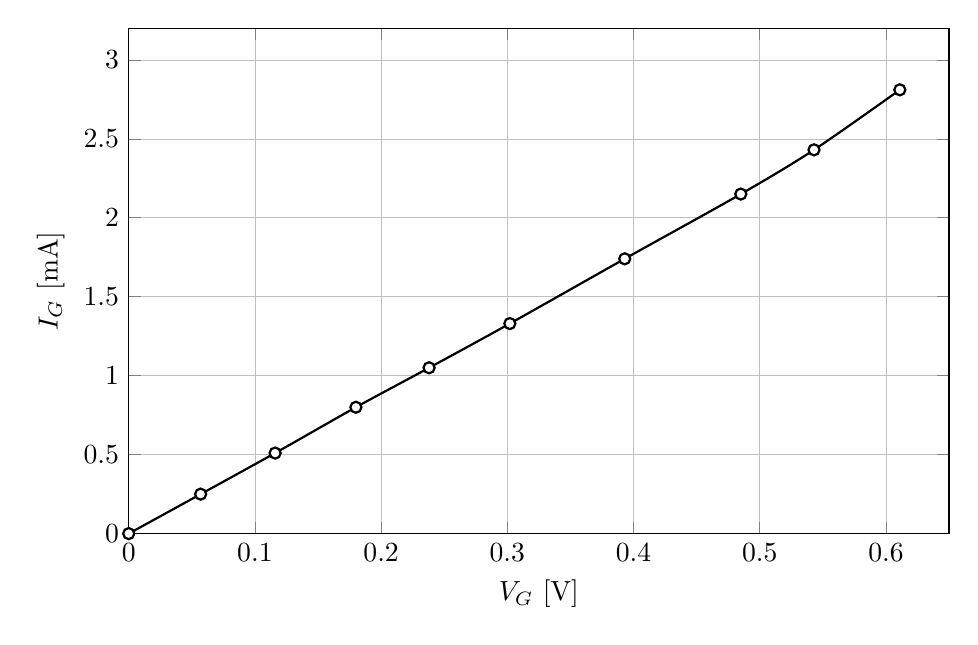
\begin{tikzpicture}
    \begin{axis}[
        width=12cm,
        height=8cm,
        xlabel={$V_G$ [V]},
        ylabel={$I_G$ [mA]},
        grid=both,
        ymin=0, ymax=3.2,
        xmin=0, xmax=0.65,
        major grid style={line width=.2pt,draw=gray!50},
        minor grid style={line width=.1pt,draw=gray!30},
        legend pos=north west
    ]

    \addplot[
        thick,
        smooth,
        mark=*,
        mark options={fill=white},
    ] coordinates {
        (0,0)
        (0.057,0.25)
        (0.116,0.51)
        (0.18,0.80)
        (0.238,1.05)
        (0.302,1.33)
        (0.393,1.74)
        (0.485,2.15)
        (0.543,2.43)
        (0.611,2.81)
    };

    \end{axis}
    \end{tikzpicture}
    \caption{Curva característica $I_G$ en función de $V_G$.}
    \label{fig:ig-vg}
\end{figure}


\subsection{Actividad de simulación}

\section{Obtención de curva característica}
\subsection{Actividad de laboratorio}
Con el mismo circuito de la Fig. \ref{fig:circuito-scr}

\begin{table}[ht!]
    \centering
    \small
    \begin{tabular}{|c|c|c|c|}
       \hline
       $I_G$ [mA] & $V_{CC}$ [V] & $I_{AK}$ [mA] & $V_{AK}$ [V] \\
       \hline
        2.92 & 600 & 127.51 & 0.7 \\
        2.96 & 465 & 98.79 & 0.7 \\
        2.98 & 398 & 84.53 & 0.7 \\
        3.00 & 345 & 73.25 & 0.7 \\
        3.02 & 295 & 62.62 & 0.7 \\
       \hline
    \end{tabular}
    \caption{relevamiento de disparo del SCR para diferentes valores de $I_G$.}
\end{table}

\begin{table}[h]
    \centering
    \resizebox{\textwidth}{!}{
    \begin{tabular}{|cc|cc|cc|cc|cc|}
        \hline
        \multicolumn{2}{|c|}{$I_{G} = 2.92mA\,$}
        & \multicolumn{2}{c|}{$I_{G} = 2.96mA\,$}
        & \multicolumn{2}{c|}{$I_{G} = 2.98mA\,$}
        & \multicolumn{2}{c|}{$I_{G} = 3.00mA\,$}
        & \multicolumn{2}{c|}{$I_{G} = 3.02mA\,$}\\
        \hline
        $V_{AK}$ [V] & $I_{AK}$ [mA] & $V_{AK}$ [V] & $I_{AK}$ [mA] & $V_{AK}$ [V] & $I_{AK}$ [mA] & $V_{AK}$ [V] & $I_{AK}$ [mA] & $V_{AK}$ [V] & $I_{AK}$ [mA] \\
        \hline
        0    & 0.000  & 0      & 0.000  & 0     & 0.000 & 0     & 0.000& 0    & 0.000 \\
        50   & 0.000  & 50     & 0.000  & 50    & 0.000 & 50    & 0.000& 50   & 0.000 \\
        100  & 0.000  & 98     & 0.000  & 100   & 0.000 & 100   & 0.000& 98.3 & 0.000 \\
        200  & 0.000  & 148    & 0.000  & 147.5 & 0.000 & 148.2 & 0.000& 148  & 0.000 \\
        300  & 0.000  & 197.5  & 0.000  & 198   & 0.000 & 200   & 0.000& 200  & 0.000 \\
        350  & 0.000  & 247.5  & 0.000  & 250   & 0.000 & 247   & 0.000& 247.5& 0.638\\
        400  & 0.000  & 296.1  & 0.000  & 296.3 & 0.000 & 297   & 0.000& 297.5& 0.53 \\
        450  & 0.000  & 343.5  & 0.000  & 346   & 0.000 & 320.8 & 0.89 & 0.7  & 62.62 \\
        500  & 0.000  & 392.4  & 0.000  & 0.7   & 84.53 & 0.7   & 73.25  & -  &- \\
        550  & 0.000  & 443.6  & 0.000  & -     & -     & -   & - & - & - \\
        600  & 0.000  & 0.7    & 98.79  & -     & -     & -   & - & - & - \\
        0.7 & 127.51 &-&-&-&-&-&-&-&-\\
        \hline
    \end{tabular}
    }
    \caption{Tabla de $I_{AK} = f(V_{AK})$ para distintos valores de $I_{G}$.}
\end{table}

\begin{figure}[h]
    \centering
    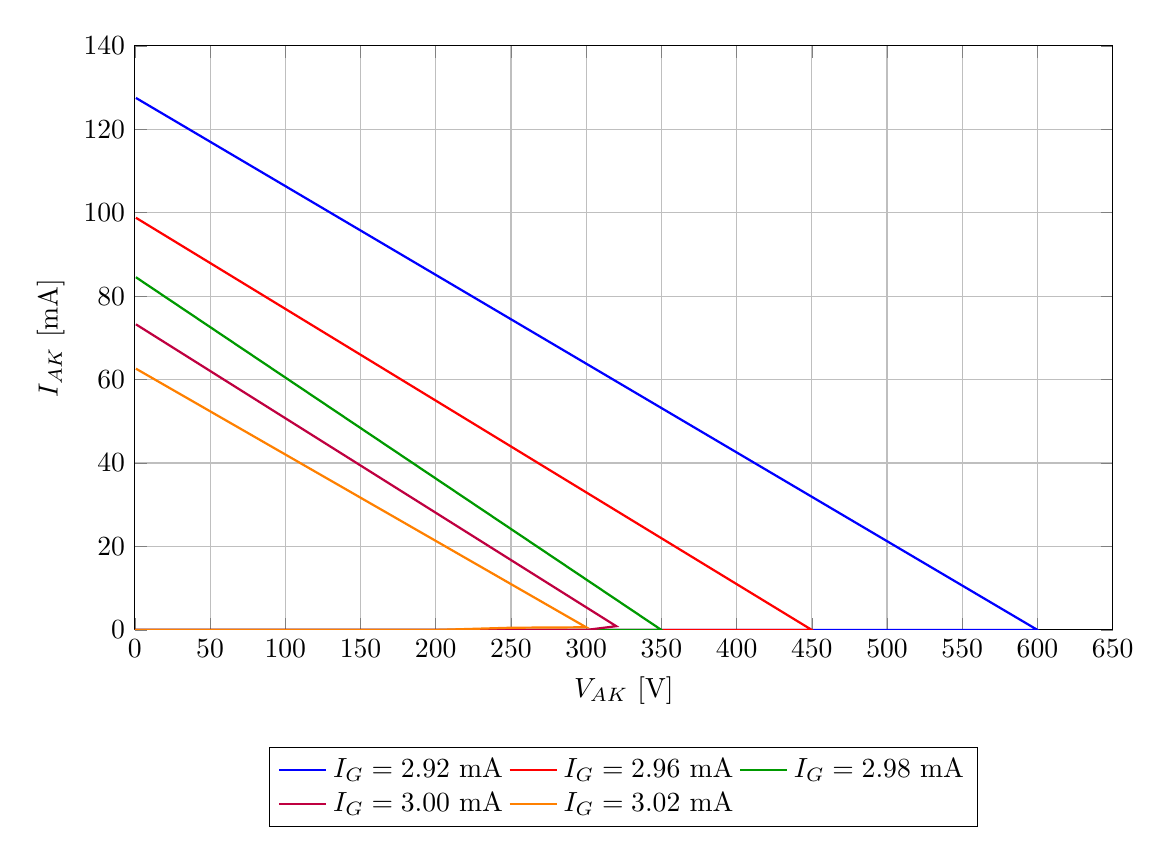
\begin{tikzpicture}
    \begin{axis}[
        width=14cm,
        height=9cm,
        xlabel={$V_{AK}$ [V]},
        ylabel={$I_{AK}$ [mA]},
        grid=both,
        ymin=0, ymax=140,
        xmin=0, xmax=650,
        legend style={at={(0.5,-0.2)},anchor=north,legend columns=3},
    ]

    % ---- IG = 2.92 mA ----
    \addplot[blue, thick] coordinates {
        (0,0) (50,0) (100,0) (200,0) (300,0) (400,0) (500,0) (600,0)
        (0.7,127.51)
    };
    \addlegendentry{$I_G = 2.92$ mA}

    % ---- IG = 2.96 mA ----
    \addplot[red, thick] coordinates {
        (0,0) (50,0) (100,0) (150,0) (200,0) (250,0) (300,0)
        (350,0) (400,0) (450,0) (0.7, 98.79)
    };
    \addlegendentry{$I_G = 2.96$ mA}

    % ---- IG = 2.98 mA ----
    \addplot[green!60!black, thick] coordinates {
        (0,0) (50,0) (100,0) (150,0) (200,0) (250,0) (300,0) (350,0) (0.7,84.53)
    };
    \addlegendentry{$I_G = 2.98$ mA}

    % ---- IG = 3.00 mA ----
    \addplot[purple, thick] coordinates {
        (0,0) (50,0) (100,0) (150,0) (200,0) (250,0) (300,0) (320,0.9)
        (0.7,73.25)
    };
    \addlegendentry{$I_G = 3.00$ mA}

    % ---- IG = 3.02 mA ----
    \addplot[orange, thick] coordinates {
        (0,0) (50,0) (100,0) (150,0) (200,0) (250,0.53) (300,0.638)
        (0.7,62.62)
    };
    \addlegendentry{$I_G = 3.02$ mA}

    \end{axis}
\end{tikzpicture}
\caption{Curvas características $I_{AK}(V_{AK})$ del SCR para distintos $I_G$.}
\end{figure}



\section{Funcionamiento con corriente alterna}
\subsection{Actividad de simulación}

\chapter{DIAC}
Objetivo: determinar la polarización y funcionamiento del DIAC.
\section{Actividad de laboratorio}
\begin{figure}[ht!]
    \centering
    \begin{tikzpicture}
        % Paths, nodes and wires:
        \draw (-1.75, -1) to[full bidirectionaldiode] (-1.75, 1);
        \draw (1.25, -1) to[voltmeter, l={$V_2$}] (1.25, 1);
        \draw (-1.75, 1) to[american resistor, l={$R$}] (-1.75, 3);
        \node[vcc](N1) at (-1.75, 3.5){} node[anchor=south] at (N1.text){$V_{CC}$};
        \draw (-1.75, 1) -- (1.25, 1);
        \draw (-1.75, -1) -- (1.25, -1);
        \draw (3.25, -0) to[voltmeter, l={$V_1$}] (3.25, 2);
        \draw (-1.75, 3) -| (3.25, 2);
        \draw (-1.75, -3) to[ammeter] (-1.75, -1);
        \node[ground] at (-1.75, -3){};
        \draw (-1.75, 3) -| (-1.75, 3.5);
        \draw (3.25, -0) |- (-1.75, -1.25);
    \end{tikzpicture}
    \caption{circuito implementado en el laboratorio.}
\end{figure}

\begin{table}[ht!]
    \centering
    \small
    \begin{tabular}{|c|c|c|c|c|c|c|c|c|c|}
       \hline
       $V_{CC}$ [V] & 0 & 10 & 20 & 30 & 32 & 34 & 40 & 45 & 50 \\
       \hline
       $V_{AK}$ [V] & 0 & 10 & 20 & 30 & 23.8 & 23.4 & 22.6 & 22.2 & 21.9 \\
       \hline
       $I_{AK}$ [mA] & 0 & 0 & 0 & 0 & 1.74 & 2.24 & 3.72 & 4.9 & 5.92 \\
       \hline
    \end{tabular}
    \caption{relevamiento de disparo del SCR para diferentes valores de $I_G$.}
\end{table}

\begin{figure}[ht!]
  \centering
  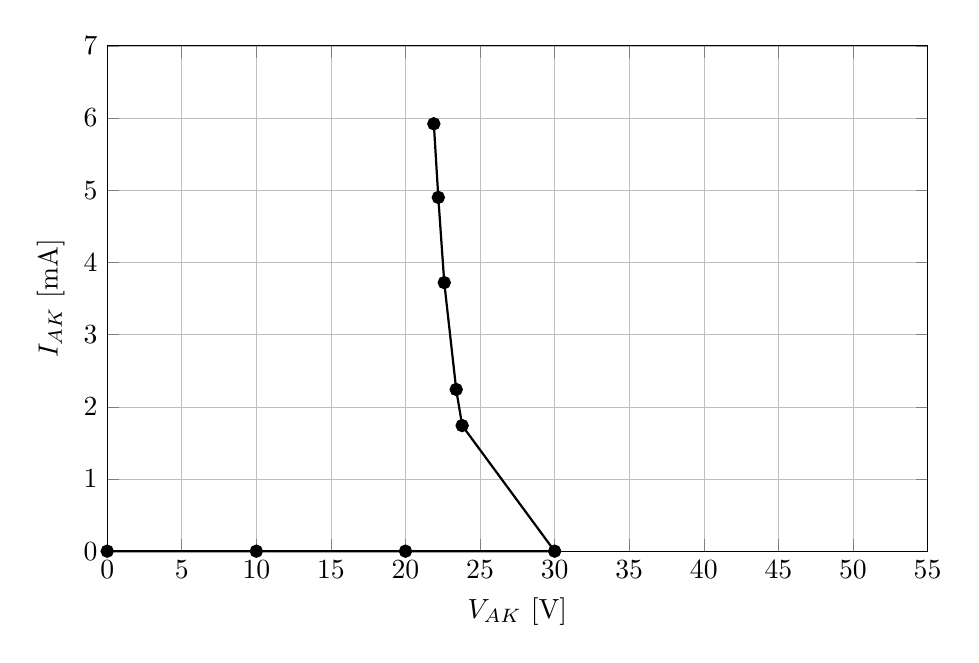
\begin{tikzpicture}
    \begin{axis}[
      width=12cm, height=8cm,
      xlabel={$V_{AK}$ [V]},
      ylabel={$I_{AK}$ [mA]},
      xmin=0, xmax=55,
      ymin=0, ymax=7,
      grid=both,
      grid style={line width=.1pt, draw=gray!30},
      major grid style={line width=.2pt,draw=gray!50},
      legend pos= north west,
      enlargelimits=false,
      clip=false,
    ]

    % Datos (ordenados para la gráfica)
    \addplot[
      mark=*,
      mark options={fill=white},
      thick,
    ] coordinates {
      (0,0)
      (10,0)
      (20,0)
      (30,0)
      (23.8,1.74)
      (23.4,2.24)
      (22.6,3.72)
      (22.2,4.90)
      (21.9,5.92)
      };

    % Marcar los puntos originales (más visibles)
    \addplot[only marks, mark=*, mark size=2pt] coordinates {
      (0,0) (10,0) (20,0) (21.9,5.92) (22.2,4.90) (22.6,3.72)
      (23.4,2.24) (23.8,1.74) (30,0) 
    };

    \end{axis}
  \end{tikzpicture}
  \caption{Curva $I_{AK}$ vs $V_{AK}$ del DIAC (datos experimentales).}
  \label{fig:diac-IV}
\end{figure}

\chapter{TRIAC}
\section{Polarización y funcionamiento}
\subsection{Actividad de laboratorio}
\begin{figure}[ht]
    \centering
    \begin{tikzpicture}
        % Paths, nodes and wires:
        \draw (0.02, 2) to[american resistor, l={$R$}] (0.02, 4);
        \node[ground] at (0.02, -3.7){};
        \draw (-1.253, -0.018) to[full bidirectionaldiode] (-3.253, -0.018);
        \draw (0, -1.75) to[full triac] (0.02, 0.3);
        \draw (-5, -0) to[ammeter, l={$I_G$}] (-3.5, -0);
        \draw (-6, -1) to[american potentiometer, mirror] (-6, 1);
        \draw (0.02, 0.3) |- (0, 2);
        \draw (-6, 1) -- (-6, 2) -- (0, 2);
        \draw (0.02, -3.7) to[ammeter, l={$I_A$}] (0, -1.75);
        \draw (2.25, -2) to[voltmeter, l={$V_{CC}$}] (2.25, 1);
        \draw (2.25, -2) |- (0.02, -3.7);
        \draw (2.25, 1) |- (0.02, 4);
        \draw (-6, -1) |- (0.02, -3.7);
        \node[vcc] at (0, 4){};
        \node[vcc](N1) at (0.02, 4){} node[anchor=south] at (N1.text){$V_{CC}$};
        \draw (-5, -0) -- (-5.44, -0);
        \draw (-3.25, -0) -- (-3.5, -0);
        \draw (-1.253, -0.018) -- (-0.753, -0.018);
    \end{tikzpicture}
    \caption{circuito implementado en el laboratorio.}
\end{figure}


% ===== PREÁMBULO (lo que pediste) ===========================================
% \usepackage[utf8]{inputenc}
% \usepackage{array}
% \usepackage[table]{xcolor}
% \usepackage{colortbl}
% \usepackage{caption}
% \usepackage{graphicx}
% \usepackage{amsmath}
% \usepackage{multirow}
% \usepackage{float}
% \usepackage{geometry} % [a4paper,margin=2.5cm]
% \newcommand{\widemargins}{\newgeometry{left=1.5cm,right=1.5cm,top=1.8cm,bottom=1.8cm}}
% \usepackage{pgfplots}
% \pgfplotsset{compat=1.18}
% ============================================================================

% ---- Etiquetas de tensiones (editables si cambiara algo) -------------------
\newcommand{\VCCA}{80}
\newcommand{\VCCB}{130}
\newcommand{\VCCC}{180}

% ========================== TABLA DE MEDICIONES =============================
\begin{table}[H]
\centering
\setlength{\tabcolsep}{5pt}
\renewcommand{\arraystretch}{1.12}
\rowcolors{2}{black!3}{white}
\begin{tabular}{
c|*{2}{>{\centering\arraybackslash}p{1.6cm}}|
  *{2}{>{\centering\arraybackslash}p{1.6cm}}|
  *{2}{>{\centering\arraybackslash}p{1.6cm}}}
\rowcolor{black!8}
\multicolumn{1}{c|}{$V_1$ [V]} &
\multicolumn{2}{c|}{$V_{CC}=\VCCA$ V} &
\multicolumn{2}{c|}{$V_{CC}=\VCCB$ V} &
\multicolumn{2}{c}{$V_{CC}=\VCCC$ V} \\
\rowcolor{black!8}
 & $I_G$ [$\mu$A] & $I_A$ [mA] & $I_G$ [$\mu$A] & $I_A$ [mA] & $I_G$ [$\mu$A] & $I_A$ [mA] \\
\hline
0    & 0    & 0    & 0    & 0    & 0 & 0 \\
5    & 0    & 0    & 0    & 0    & 0 & 0 \\
10   & 0    & 0    & 0    & 0    & 0 & 0 \\
15   & 0    & 0    & 0    & 0    & 0 & 0 \\
20   & 0    & 0    & 0    & 0    & 0 & 0 \\
25   & 0    & 0    & 0    & 0    & 0 & 0 \\
30   & 0    & 0    & 0    & 0    & 0 & 0 \\
31   & 0    & 0    & 0    & 0    & 0 & 0 \\
31.6 &      &      & 4.53 & 4.57 &   &   \\
32   & 3.4  & 3.4  &      &      & 0 & 37.1 \\
33.0 & 3.8  & 3.9  &      &      &   &   \\
33.1 & 4.15 & 4.15 &      &      &   &   \\
33.2 & 4.6  & 4.8  &      &      &   &   \\
33.3 & 4.7  & 6.2  &      &      &   &   \\
23.4 &      &      & 4.53 & 4.57 &   &   \\
23.3 & 3.8  & 3.9  &      &      &   &   \\
23.1 & 4.15 & 4.15 &      &      &   &   \\
23.2 & 4.6  & 4.8  &      &      &   &   \\
23.7 & 4.3  & 6.0  &      &      &   &   \\
0.3  &      &      & 0    & 26.7 &   &   \\
50   &      &      &      &      & 0 & 0 \\
0    & 0    & 16.3 &      &      &   &   \\
\end{tabular}
\caption{Relevamiento de puntos para el trazado de $I_A=f(I_G)$ con tres valores de $V_{CC}$.}
\end{table}

% ===================== GRÁFICO IA = f(IG) EN EL MISMO EJE ===================
% Cargamos exactamente los pares (IG, IA) medidos para cada VCC.
\begin{figure}[H]
\centering
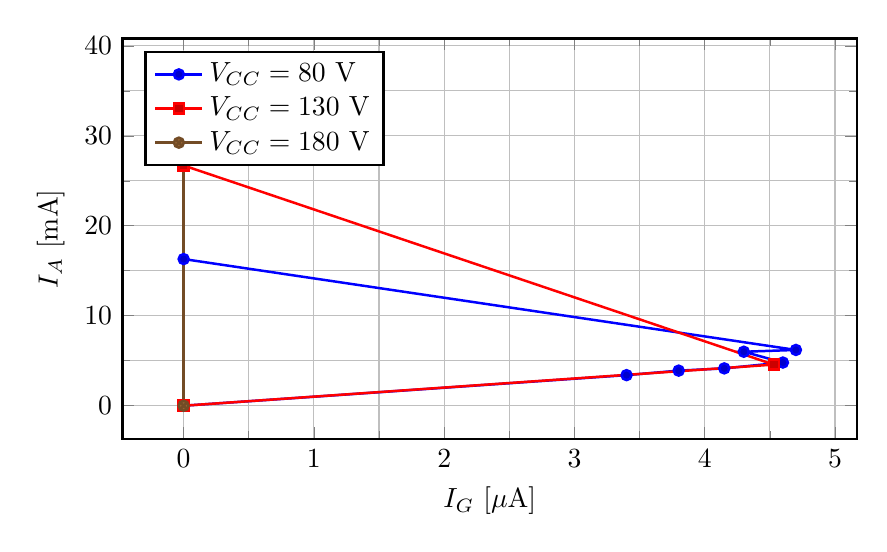
\begin{tikzpicture}
\begin{axis}[
  width=0.9\linewidth, height=0.55\linewidth,
  xlabel={$I_G$ [$\mu$A]}, ylabel={$I_A$ [mA]},
  grid=both, minor tick num=1,
  legend pos=north west, legend cell align=left,
  line width=0.9pt, mark=*, mark size=1.8pt,
]
  % ---- VCC = 80 V ----------------------------------------------------------
  \addplot+ coordinates {
    (0,0)
    (3.4,3.4)
    (3.8,3.9)
    (4.15,4.15)
    (4.6,4.8)
    (4.3,6.0)
    (4.7,6.2)
    (0,16.3) % punto de mantenimiento/latch observado
  };
  \addlegendentry{$V_{CC}=80$ V}

  % ---- VCC = 130 V ---------------------------------------------------------
  \addplot+ coordinates {
    (0,0)
    (4.53,4.57)
    (4.53,4.57) % repetido porque aparece en dos V1 distintos
    (0,26.7)
  };
  \addlegendentry{$V_{CC}=130$ V}

  % ---- VCC = 180 V ---------------------------------------------------------
  \addplot+ coordinates {
    (0,0)
    (0,37.1)
  };
  \addlegendentry{$V_{CC}=180$ V}
\end{axis}
\end{tikzpicture}
\caption{Curvas características $I_A=f(I_G)$ para $V_{CC}\in\{80,130,180\}\,\mathrm{V}$.}
\end{figure}

% =============================== CONCLUSIONES ===============================
\noindent\textbf{Conclusiones.}
Las curvas $I_A=f(I_G)$ muestran un umbral de disparo $I_{G,\text{th}}$: por debajo de ese valor
la conducción es nula; superado, $I_A$ crece con alta pendiente (modo de disparo/latch).
Con mayor $V_{CC}$, el dispositivo sostiene corrientes de ánodo más grandes para valores similares
de $I_G$, y el mantenimiento de conducción (holding) aparece a corrientes mayores. Los puntos
$(I_G{=}0,\ I_A{>}0)$ registrados en $V_{CC}=80$ y $180~\mathrm{V}$ evidencian el estado
mantenido tras el disparo. La región cercana al umbral presenta mayor dispersión, esperable por
tolerancias y efectos térmicos. En síntesis, los datos son consistentes con el mecanismo de disparo
y su dependencia con la tensión de alimentación.














\section{Aplicación: control de disparo (Dimmer)}
\subsection{Actividad de laboratorio}
\subsection{Análisis de las gráficas relevadas}
En el dimmer con DIAC--TRIAC, el ángulo de disparo $\alpha$ lo fija la constante de tiempo
$RC$ del circuito de compuerta. Al aumentar el valor del potenciómetro, crece $\tau=RC$ y
la tensión del capacitor tarda más en alcanzar el \emph{breakover} del DIAC ($\approx 30$ V),
por lo que $\alpha$ aumenta y la potencia en la carga disminuye.

De las tres capturas oscilográficas:
\begin{itemize}
  \item \textbf{Potenciómetro al máximo (mayor $R$):} la conducción inicia tarde en cada
        semiciclo ($\alpha$ grande). La forma de onda en la carga muestra «rebanado»
        de los primeros grados y un valor eficaz bajo.
  \item \textbf{Posición intermedia:} $\alpha$ medio. El intervalo de conducción crece y
        el valor eficaz sube. La salida mantiene simetría entre semiciclos gracias al DIAC.
  \item \textbf{Potenciómetro al mínimo (menor $R$):} $\alpha$ pequeño, se aprovecha casi todo
        el semiciclo. La tensión eficaz de carga se aproxima a la de la red.
\end{itemize}
En los tres casos el TRIAC se apaga al final de cada semiciclo cuando la corriente
instantánea cae por debajo de la corriente de mantenimiento $I_H$; se observa un
\emph{cierre} cercano al cruce por cero.

\subsection{Dependencia de $I_H$ con $I_G$, $V_G$ y $V_{CC}$}
\paragraph{Definición práctica.}
Con carga resistiva $R_L$ y tensión de pico $V_m$, una vez disparado el TRIAC, la corriente
de carga vale $i(t)=\dfrac{V_m}{R_L}\sin(\omega t)$ (desfasada por $\alpha$). El apagado se
produce cuando $|i(t)|=I_H$. De aquí:
\[
  \omega t_{\mathrm{off}} = \arcsin\!\left(\frac{I_H R_L}{V_m}\right), \qquad
  \beta = \omega t_{\mathrm{off}}, \qquad
  I_H = \frac{V_m}{R_L}\,\sin\beta,
\]
donde $\beta$ es el ángulo de apagado medido en la oscilografía (el instante en que la
tensión de carga vuelve a cero).

\paragraph{Relación con $I_G$ y $V_G$.}
$I_H$ es un parámetro del dispositivo y \emph{no depende} del disparo una vez que el TRIAC
está en conducción. $I_G$ y $V_G$ sólo afectan \emph{cuándo} se dispara (el valor de
$\alpha$), no el umbral de mantenimiento. Pueden existir efectos indirectos: un disparo con
pulso de compuerta más intenso incrementa la potencia media y la temperatura de juntura, y
$\,I_H$ suele presentar ligera dependencia con $T_J$ (según hoja de datos). Ese efecto es
secundario frente a la dependencia dominante con la corriente de carga instantánea.

\paragraph{Relación con $V_{CC}$.}
A mayor $V_{CC}$ (mayor $V_m$), para un mismo $R_L$ la corriente de carga es mayor y el
criterio $|i|=I_H$ se alcanza más cerca del cruce por cero, por lo que la conducción se
extiende un poco más dentro del semiciclo. De la ecuación anterior:
\[
  \beta = \arcsin\!\left(\frac{I_H R_L}{V_m}\right),
\]
se ve que $\beta$ \emph{disminuye} al aumentar $V_m$ (el TRIAC se mantiene conduciendo
hasta un ángulo más próximo a $\pi$).

\paragraph{Procedimiento de extracción de $I_H$ (usado en el laboratorio).}
\begin{enumerate}
  \item Medir en el osciloscopio el instante de apagado por semiciclo y leer la tensión de
        carga $v_L(t_{\mathrm{off}})$.
  \item Calcular $i(t_{\mathrm{off}})=v_L(t_{\mathrm{off}})/R_L$; ese valor es $I_H$.
  \item Alternativamente, medir el ángulo $\beta$ y usar $I_H=\dfrac{V_m}{R_L}\sin\beta$.
\end{enumerate}

\subsection{Conclusiones}
\begin{itemize}
  \item El control de potencia se logra variando $\alpha$ mediante la constante de tiempo
        $RC$; la presencia del DIAC asegura disparo simétrico y reduce armónicos pares.
  \item $I_H$ fija el \emph{apagado natural} por semiciclo y es mayormente independiente
        de $I_G$ y $V_G$ una vez establecido el régimen de conducción.
  \item El aumento de $V_{CC}$ incrementa la corriente de carga y retrasa (angularmente)
        el cumplimiento de $|i|=I_H$, extendiendo levemente el intervalo de conducción.
  \item Las mediciones concuerdan con el modelo: las formas de onda muestran recorte
        controlado al inicio del semiciclo y apagado próximo al cruce por cero.
\end{itemize}








\clearpage
\widemargins

\chapter{Interpretación de las especificaciones del fabricante}


\section{DIAC (DB3)}
Dispositivo bidireccional de disparo por tensión (\emph{breakover}). Conduce cuando la tensión
entre sus terminales supera $V_{BO}$ (en cualquiera de las dos polaridades) y luego cae a un valor
menor por el \emph{breakback} dinámico.

\begin{table}[h]
  \centering
  \setlength{\tabcolsep}{4pt}
  \renewcommand{\arraystretch}{1.15}
  \begin{tabular}{lclp{0.25\linewidth}}
    \hline
    Parámetro & Símbolo & Valor (DB3) & Significado \\
    \hline
    Tensión de disparo & $V_{BO}$ & 32\,V típ; 28--36\,V & Tensión a la que el DIAC entra en conducción. \\
    Simetría de $V_{BO}$ & $|V_{BO1}|-|V_{BO2}|$ & $\le 3$\,V & Diferencia de $V_{BO}$ entre semicírculos. \\
    Corriente de disparo & $I_{BO}$ & $\le 50$\,mA & Corriente al momento del disparo. \\
    Breakback dinámico & $\Delta V$ & $\le 5$\,V & Caída de tensión inmediata luego del disparo. \\
    Corriente pico en pulso & $I_C$ & 2.0\,A (10\,ms, 120\,pps) & Límite de corriente de pico permitida. \\
    \hline
  \end{tabular}
\end{table}

\section{SCR (C106)}
Tiristor unidireccional. Se dispara con corriente de compuerta $I_{GT}$ o por sobrepaso de $dV/dt$,
y se mantiene conduciendo mientras $I_T \ge I_H$.

\begin{center}
\begin{tabular}{lclp{0.20\linewidth}}
\hline
Parámetro & Símbolo & Valor & Significado \\
\hline
Tensión de bloqueo rep. & $V_{DRM},V_{RRM}$ & 200/400/600\,V & Máx. tensión repetitiva en estado de corte (F/R). \\
Corr.\ on--state (RMS) & $I_{T(RMS)}$ & 4.0\,A & Corriente eficaz admisible a 80$^\circ$C. \\
Corr.\ on--state (prom.) & $I_{T(AV)}$ & 2.55\,A & Corriente promedio para 180$^\circ$ (a 80$^\circ$C). \\
Corriente de sobrecarga & $I_{TSM}$ & 20\,A & Pico no repetitivo (1/2 ciclo, 60\,Hz, $T_J{=}110^\circ$C). \\
Corr.\ de fuga & $I_{DRM},I_{RRM}$ & 10/100\,$\mu$A & Fuga a $V_{DRM}/V_{RRM}$, 25/110$^\circ$C. \\
Corr.\ disparo de compuerta & $I_{GT}$ & 15--35\,$\mu$A típ; $\le$200--500\,$\mu$A & Corriente mínima en compuerta para disparo. \\
Tensión de compuerta & $V_{GT}$ & 0.4--0.8\,V típ; $\le 1.0$\,V & Tensión en compuerta al disparo. \\
Tensión on--state & $V_T$ ($V_{TM}$) & $\le 2.2$\,V (@ 4\,A) & Caída directa en conducción. \\
Corriente de enganche & $I_L$ & 0.20--0.35\,mA típ & Corriente mínima para quedar enganchado tras disparo. \\
Corriente de mantenimiento & $I_H$ & 0.07--0.33\,mA típ; $\le 2$--6\,mA & Corriente mínima para sostener conducción. \\
Resistencia térmica j--c & $R_{\theta JC}$ & 3.0\,$^\circ$C/W & De unión a cápsula. \\
Resistencia térmica j--a & $R_{\theta JA}$ & 75\,$^\circ$C/W & De unión a ambiente. \\
Tiempo de encendido & $t_{gt}$ & \emph{No especificado} & Tiempo controlado por compuerta hasta conducción. \\
Tiempo de apagado & $t_q$ & \emph{No especificado} & Intervalo tras la conmutación para recuperar bloqueo. \\
\hline
\end{tabular}
\end{center}

\section{TRIAC (BT136)}
Tiristor bidireccional (dos SCR anti-serie con compuerta común). Se dispara en cuatro cuadrantes;
parámetros dependen de la variante (\mbox{-500/-600/-800}) y del cuadrante de disparo.

\begin{center}
\begin{tabular}{lclp{0.20\linewidth}}
\hline
Parámetro & Símbolo & Valor & Significado \\
\hline
Tensión de bloqueo rep. & $V_{DRM},V_{RRM}$ & 500/600/800\,V & Tensión repetitiva en corte. \\
Corr.\ on--state (RMS) & $I_{T(RMS)}$ & 4.0\,A & A $T_{mb}\le 107^\circ$C, onda senoidal. \\
Corriente de sobrecarga & $I_{TSM}$ & 25\,A (20\,ms); 27\,A (16.7\,ms) & Pico no repetitivo. \\
Corriente de compuerta & $I_{GT}$ & 5--100\,mA según cuadrante/serie & Mínima corriente de disparo. \\
Tensión de compuerta & $V_{GT}$ & 0.7--1.5\,V & Tensión en compuerta al disparo. \\
Corriente de mantenimiento & $I_H$ & 5--30\,mA & Corriente mínima para sostener conducción. \\
Tensión on--state & $V_T$ & 1.4\,V típ; 1.7\,V máx (@ 5\,A) & Caída en conducción. \\
Tiempo de encendido & $t_{gt}$ & $\le 2\,\mu$s & Tiempo controlado por compuerta hasta conducción. \\
Tiempo de apagado & $t_q$ & \emph{No especificado} & En TRIAC se usan d$V$/dt y d$I$/dt de conmutación. \\
Resistencia térmica j--mb & $R_{\theta j\mbox{-}mb}$ & 3.0\,K/W (ciclo completo) & Unión a base de montaje. \\
Resistencia térmica j--a & $R_{\theta j\mbox{-}a}$ & 60\,K/W (aire libre) & Unión a ambiente. \\
Temp.\ de almacenamiento & $T_{STG}$ & $-40$ a $+150^\circ$C & Rango de almacenamiento. \\
Temp.\ de juntura & $T_J$ & $- \; a \; +125^\circ$C (operación) & Límite de operación de la juntura. \\
\hline
\end{tabular}
\end{center}

\subsubsection*{Notas de uso/medición}
\begin{itemize}
  \item $V_{DRM}/V_{RRM}$ se ensayan con fuente senoidal 50--60\,Hz. En TRIAC, capacidades de conmutación
        se caracterizan mediante d$V_{\mathrm{com}}$/dt y d$I_{\mathrm{com}}$/dt (no siempre hay $t_q$ explícito).
  \item En TRIAC el $I_{GT}$ varía por cuadrante (T2$\pm$/G$\pm$); elegir variante (\mbox{serie F/G}) según la
        sensibilidad requerida de compuerta.
  \item $I_L$ y $I_H$ delimitan el disparo/retención: diseñar la red de disparo para
        garantizar $I_T > I_L$ durante el flanco y $I_T > I_H$ en régimen.
\end{itemize}

\restoremargins
\clearpage

\chapter{Conclusión}
\end{document}
